\chapter{Automated rejection and repair of bad trials in M/EEG}
\label{chapter:auto_reject}

Magneto-/electroencephalography (M/EEG) measure brain activity by recording magnetic/electrical signals in multiple sensors. M/EEG data is inherently noisy, which makes it necessary to combine (\textit{e.g.}, by averaging) multiple data segments (or trials). Unfortunately, trials can sometimes be contaminated due to high amplitude artifacts which can reduce the effectiveness of such strategies.

Artifact removal in M/EEG is a complex and extensively studied topic involving different types of artifact and techniques \citep{mullen2015real, vigario1997extraction, uusitalo1997signal, taulu2004suppression, de2007denoising}. However, we focus only on the problem of detecting and repairing bad trials (and sensors) which is fundamental to virtually any M/EEG analysis pipeline. In fact, even artifact rejection methods can implicitly rely on annotated bad (signal in) sensors and trials. For example, the Signal Space Separation (SSS) requires that the data has no bad sensors~\footnote{SSS partially solves this problem by automatically detecting bad sensors by removing sensors which differ from the reconstructed signal by more than a threshold.}.

Existing software for processing M/EEG data offer a simple solution by marking a trial as bad if the peak-to-peak amplitude in any sensor exceeds a certain threshold~\citep{mne}. The threshold is usually set manually after visual inspection of the data. This can turn tedious for studies involving hundreds of recordings (see the Human Connectome Project \citep{van2012human} as an example of such a large-scale study).

\begin{figure}[t]
\begin{center}
	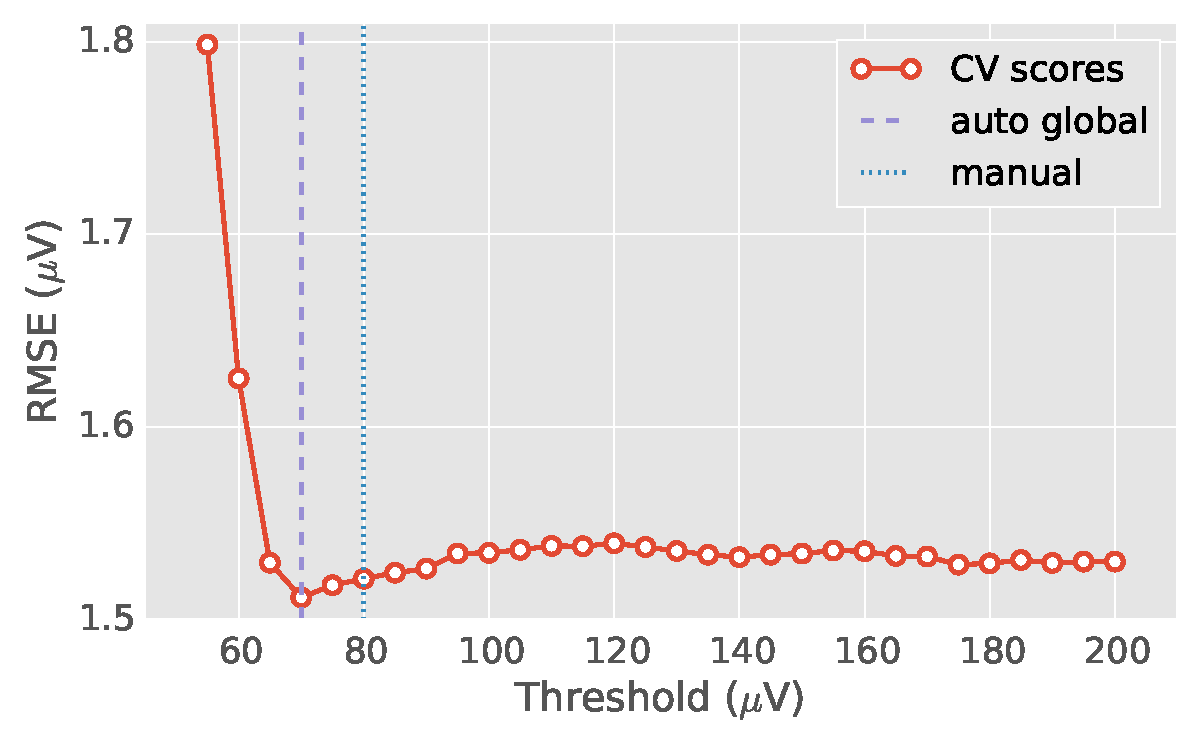
\includegraphics[width=0.7\linewidth]{figures/figure1.pdf}
\end{center}
    \caption{Mean cross-validation error as a function of peak-to-peak rejection threshold. The root mean squared error (RMSE) between the mean of the training set (after removing the trials marked as bad) and the median of the validation set was used as the cross-validation metric. The optimal data-driven  threshold (\emph{auto reject, global}) with minimum RMSE closely matches the human threshold.
 }
    \label{fig:basic_cv}
\end{figure}

\iftoggle{long}{% for journal version
Recently, there has been some progress in addressing this issue. Most of these methods depend on engineering features to describe the data statistics and rejecting data based on a tuneable threshold on these statistics. As an example, FASTER~\citep{nolan2010faster} rejects based on a threshold on the z-score of the trial variance, its amplitude range, \textit{etc}. Reimannian potato filtering~\citep{barachant2013riemannian} is yet another method which uses the covariance matrix of sensor data. Trials whose Reimannian distance  from a reference covariance matrix (estimated adaptively across time windows) is above a certain threshold, are rejected. Note that this method does not offer any insights into which sensors are artifactual. Another related method is Artifact Subspace Reconstruction~\citep{kothe2015artifact} which removes artifact components whose variance exceeds the reference data variance by more than a threshold. In all these methods, the tuneable threshold must either be set manually or remain fixed. One quickly realizes that a fixed threshold is certainly not optimal for all datasets, an issue which we address in this paper.
}{ % PRNI version
Modern algorithms for rejecting trials compute more advanced trial statistics.  FASTER~\citep{nolan2010faster}, for example, rejects based on a threshold on the z-score of the trial variance, its amplitude range, \textit{etc}. Riemannian potato filtering~\citep{barachant2013riemannian} works on covariances matrices~\citep{barachant2013riemannian} and Artifact Subspace Reconstruction~\citep{kothe2015artifact} rejects based on the variance of artifact components. However, these methods are not fully satisfactory as rejection thresholds must be fixed or manually tuned.}\iftoggle{long}{% for journal version
\par A more promising approach for detecting bad trials/sensors is to apply algorithms robust to outliers. If, for instance, the end goal of the analysis is to compute an average evoked response, one can approach this using a weighted average, e.g. robust regression \citep{diedrichsen2005detecting}. Here, interference by artifacts is mitigated by down-weighting contaminated trials in the average. While this approach is viable when computing clean averaged signals, it cannot be considered for analysis at the level of single trials. This implies that outliers must be detected at the level of single trials. The Random Sample Consensus (RANSAC) algorithm implemented as part of the PREP pipeline \citep{bigdely2015prep} can in fact detects outlier sensors at the level of single-trials.
}

At this point, the reader may note that algorithms proposed thus far treat the problem of detection bad trials or bad sensors as related but separate problems. However, considering that bad sensors in EEG data varies between runs, and even between trials, our approach is to treat them as the same problem. We propose a unified approach to detecting and interpolating bad sensors at the level of single-trials.

% First, it estimate a clean covariance matrix of the data using a robust geometric median over multiple time windows. The data in question is then decomposed into principal components. The reference variance for each principle component is computed using the cleaned covariance matrix. Components which differ from the reference variance by more than 3 (a tuneable parameter) standard deviations are then repaired using the non-artifact subspace. Note that this method requires a threshold parameter (3 by default), which must be adjusted depending on the data.

In this work, we make the following contributions. First, we offer a data-driven cross-validation framework (Figure \ref{fig:basic_cv}) to automatically set the rejection threshold. Secondly, we show that the rejection threshold is sensor-specific and varies considerably across sensors. Finally, we show that taking into account this variation in sensor-specific thresholds can in fact lead to improved detection and repair of bad trials. Our approach unifies rejection of bad trials and repair of bad sensors in a single method.
